% !TEX encoding = UTF-8
% !TEX TS-program = pdflatex
% !TEX root = ../tesi.tex

%**************************************************************
\chapter{Infrastruttura Preesistente e tecnologie coinvolte}
\label{cap:descrizione-architettura}
%**************************************************************

\intro{In questo capitolo verrà descritta l'architettura software del gestionale SAP e dei moduli aggiunti dall'azienda}\\
%**************************************************************
\begin{figure}[!h] 
	\centering 
	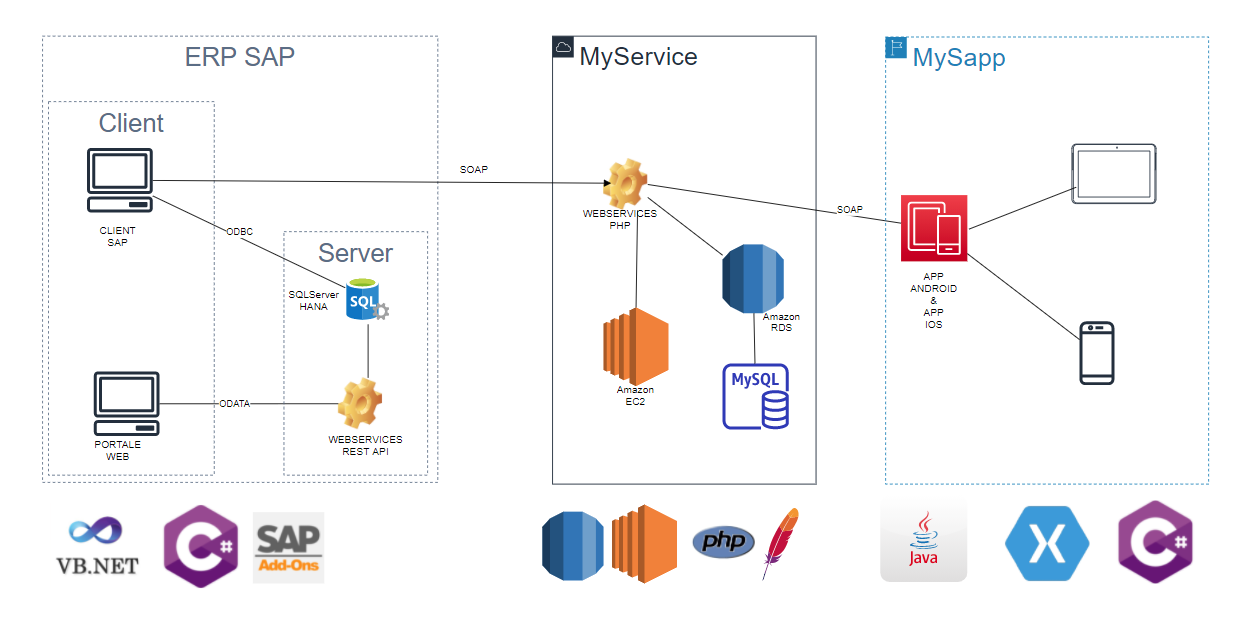
\includegraphics[scale = 0.4]{immagini/architettura-globale.png} 
	\caption{Schema di rappresentazione modulo gestionale ERP SAP, e moduli aggiunti dall'azienda intorno al gestionale}
	\label{fig:2-1}
\end{figure}\\
L'azienda ha una infrastruttura per collegare il gestionale a delle applicazioni smartphone ed un portale web. \\Si basa su 3 moduli che si connettono tramite protocollo \gls{soap}.
\\
Dalla figura \ref{fig:2-1} possiamo notare i tre moduli principali:
\begin{itemize}
	\item \textbf{ERP SAP:} il modulo del gestionale;
	\item \textbf{MyService:} il modulo dei webservices \gls{aws};
	\item \textbf{MySapp:} il modulo delle applicazioni Android e iOS.\\
\end{itemize}
Sulle due parti evidenziate dal cerchio rosso si è basato il mio lavoro in questo stage.
Nel client SAP verrà applicato l'applicazione add-on, mentre nei webservices php sono state effettuate delle modifiche ad alcune funzioni.
\section{Descrizione modulo ERP SAP}
\begin{figure}[!h] 
	\centering 
	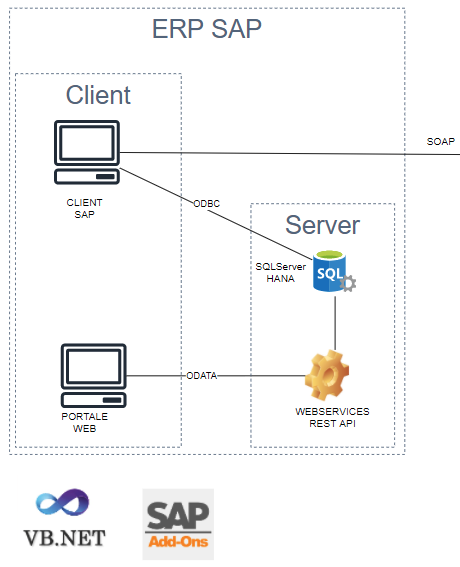
\includegraphics[scale = 1.2]{immagini/modulo-sap.png} 
	\caption{Schema di rappresentazione modulo gestionale ERP SAP}
\end{figure}

\subsection{ERP SAP}
\vspace{1em}
ERP SAP rappresenta il modulo del gestionale, in particolare nel nostro caso abbiamo come gestionale il SAP Business One.\\
ERP è l'acronimo di Enterprise Resource Planning.\\SAP è l'acronimo di Systems, Applications, Products.\\\\
SAP è un'azienda leader nel settore di ERP, e i suoi prodotti sono dei gestionali, ovvero dei software ERP.\\\\
Il gestionale SAP è un tipo di software che le organizzazioni utilizzano per gestire le attività commerciali quotidiane, come ad esempio contabilità, project management, gestione del rischio e operazioni e gestione della catena di distribuzione.\\\\
Come possiamo vedere in Figura 2.2, il SAP è suddiviso in client e server.\\
Il server può essere basato su :
\begin{itemize}
	\item \textbf{SQLServer:} solo su Windows;
	\item \textbf{HANA:} solo su Linux.
\end{itemize}
Il client SAP attualmente è disponibile solo su Windows.\\Sul client SAP possono essere applicati degli add-on, per modificare i comportamenti della GUI del client in base a com'è programmato l'add-on.\\\\
I due gestionali più famosi di SAP sono:
\begin{itemize}
	\item SAP R/3;
	\item SAP Business One.
\end{itemize}
Questo progetto di stage è stato incentrato intorno al SAP Business One, dunque ora entreremo più nel dettaglio, su quest'ultimo.
\newpage
\subsection{SAP Business One}
SAP Business One, abbreviato a SAB B1, è un sofware ERP per le piccole/medie imprese.
\\\\Questo gestionale è attualmente alla versione 10, rilasciata a marzo 2020, e rispetto al SAP R/3 consente molte più personalizzazione per essere adatto alle esigenze più disparate.
\\\\Come detto in precedenza è un tipico software con modello Client-server.
\begin{itemize}
	\item Il client è principalmente il Client SAP, o B1 Client, ma può essere anche un portale web oppure un'applicazione mobile;
	\item Il server viene eseguito su un database Microsoft SQL Server (Windows) oppure un database SAP HANA (Linux).\\
\end{itemize}
Infine, come detto in precedenza, SAB B1 consente di effettuare molte personalizzazioni (ovvero gli add-on) utilizzando \textbf{SAP Business One SDK}, ovvero un insieme di strumenti e librerie disponibili per lo sviluppo di add-ons su Microsoft Visual Studio, con C\# o VB.NET.\\\\
\begin{figure}[!h] 
	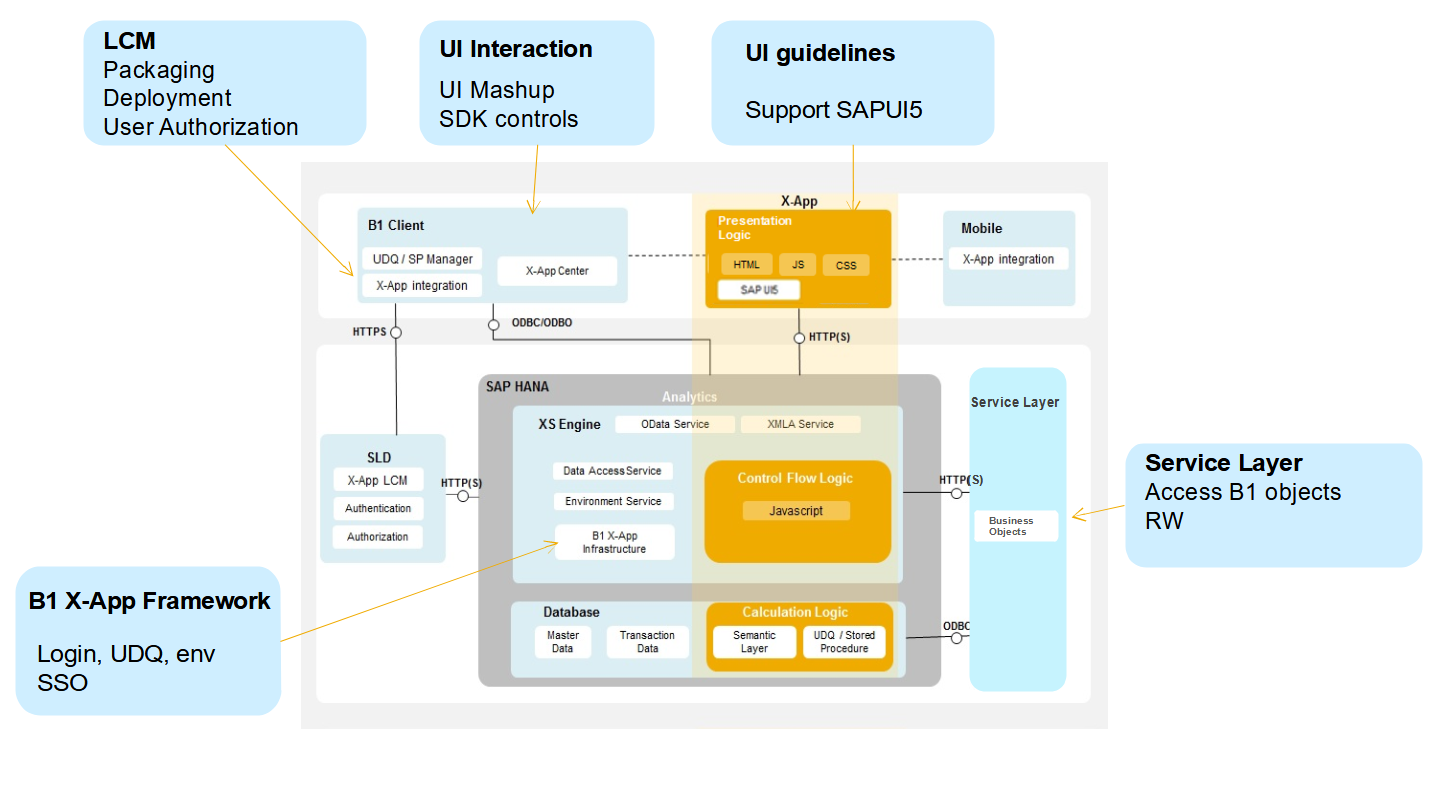
\includegraphics[scale = 0.4, left]{immagini/erp-sap-inside.png} 
	\caption{Schema ufficiale sul SAP Business One}
	\label{fig:2-3}
\end{figure}
\newpage
\begin{flushleft}
	Nella figura \ref{fig:2-3} possiamo vedere uno schema sul SAP Business One, ufficiale dalla documentazione SAP.\\
	Possiamo vedere i vari client con cui accedere al SAP:
\end{flushleft}

\begin{itemize}
	\item \textbf{B1 Client:} ovvero il client SAP desktop;
	\item \textbf{X-APP:} ovvero un portale web sviluppato da SAP;
	\item \textbf{X-APP per mobile:} l'integrazione X-APP, per i dispositivi mobile;
	\item \textbf{Service Layer:} i webservices REST API, che possono essere utilizzati a loro volta da altre applicazioni (ad esempio, sito web o applicazioni mobile), per accedere al SAP.
\end{itemize}
Tutti questi client accedono al SAP attraverso vie diverse.
\begin{itemize}
		\item Il client SAP, B1 Client, accede al database attraverso:
		\begin{enumerate}
			\item \gls{odbc} 
			\item \gls{odbo}
		\end{enumerate}
		e successivamente accede a SLD, ovvero la componente di autenticazione, via HTTP(S);
\item I webservices accedono al server SAP attraverso HTTP(S), e ricevono risposta dal database attraverso \gls{odbc};
	\item X-APP, sia versione web che mobile, accede al server SAP, e quindi successivamente al database, attraverso HTTP(S).
\end{itemize}
Sempre nella figura \ref{fig:2-3}, si può vedere XS Engine, ovvero il server SAP (la logica SAP) e il database, contenuti dentro il DBMS SAP HANA, ma lo stesso vale se il DBMS è Microsoft SQL Server.\\
Ora proseguiamo analizzando le componenti principali del SAP, ovvero:
\begin{itemize}
	\item il client SAP;
	\item il server SAP;
	\item il Service Layer di SAP, ovvero i webservices REST API.
\end{itemize}
\newpage
\subsection{Client SAP}
\begin{flushleft}
	\item Il client SAP utilizza la connessione \gls{odbc} per comunicare con il server SAP.\\ODCB, ovvero Open DataBase Connectivity, è uno standard utilizzato per la connessione tra client e DBMS. 
	\item Mentre utilizza il protocollo \gls{soap} per comunicare con il webserver \gls{aws} del modulo MyService.
\end{flushleft}
\begin{figure}[!h] 
	\centering 
	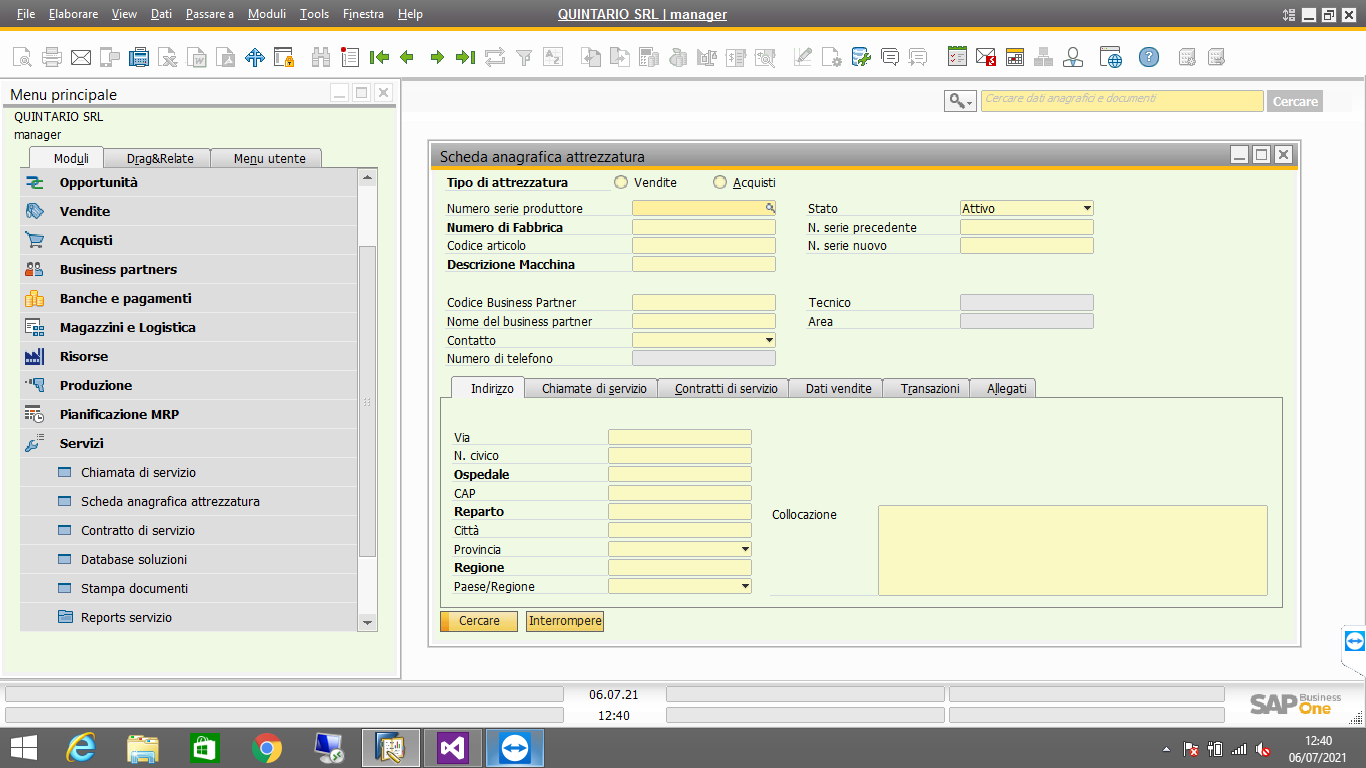
\includegraphics[scale = 0.4]{immagini/client-sap.png} 
	\caption {Client SAP, aperto sulla scheda "Scheda anagrafica attrezzatura"}
	\label{fig:2-4}
\end{figure}
\begin{flushleft}
	\item Nella figura \ref{fig:2-4} possiamo vedere come appare il Client SAP.\\In questo caso è stata aperta la Scheda anagrafica attrezzatura, del modulo dei Servizi.\\Da notare che questi "moduli" del SAP, differiscono dai moduli coinvolti con il modulo del gestionale (MyService e MySapp), questi sono moduli interni del SAP.
	\item La scheda anagrafica attrezzatura è una scheda che rappresenta le attrezzature dell'azienda, ad esempio macchine a controllo numerico, lavatrici o condizionatori, e tutti i possibili macchinari dell'azienda.
	\item Ora vediamo un esempio di cambiamento della GUI di questo client con l'applicazione di un Add-On alla scheda anagrafica attrezzatura.
\end{flushleft}
\pagebreak
\begin{figure}[!h] 
	\centering 
	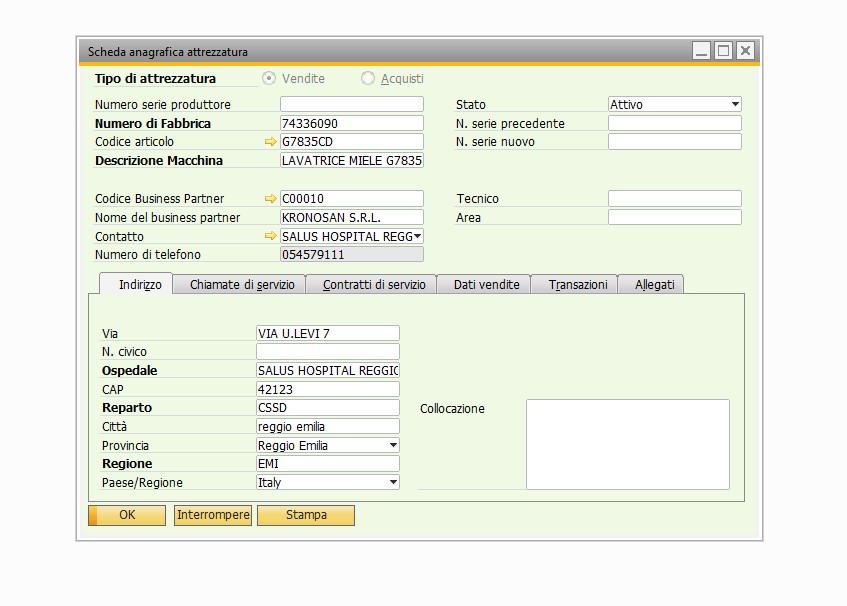
\includegraphics[scale = 0.6]{immagini/esempio-modifica-client-addon.jpg} 
	\caption {Client SAP, esempio di modifica GUI di un add-on applicato sulla scheda "Scheda anagrafica attrezzatura"}
	\label{fig:2-5}
\end{figure}
\begin{flushleft}
	\item Come possiamo vedere in figura \ref{fig:2-5} è apparso un nuovo pulsante, che stamperà i dati della scheda.\\Questo è un'esempio molto semplice, ma si possono cambiare altre cose, ad esempio aggiungere o rimuovere campi, o aggiungere funzioni ad eventi, ad esempio messaggi di testo che appaiono cliccando dei campi particolari.
	\item Questi add-on possono essere programmati tramite Microsoft Visual Studio, con :
	\begin{itemize}
		\item \textbf{C\#}, C sharp;
		\item \textbf{VB.NET}, Visual Basic NET.
	\end{itemize}
\end{flushleft}
\newpage
\subsection{Portale Web}
Ora mostriamo il portale web, sviluppato dall'azienda, in concomitanza con un'altra azienda specializzata in siti web (mys).\\
L'admin del portale, oppure l'admin relativo all'azienda cliente, crea le credenziali per i vari utenti, che saranno i dipendenti delle aziende clienti di Sinapsi.\\
Dunque arrivati al sito web, bisogna inserire le credenziali nella sezione Login, che apparirà come prima pagina del sito.\\
\begin{figure}[!h] 
	\centering 
	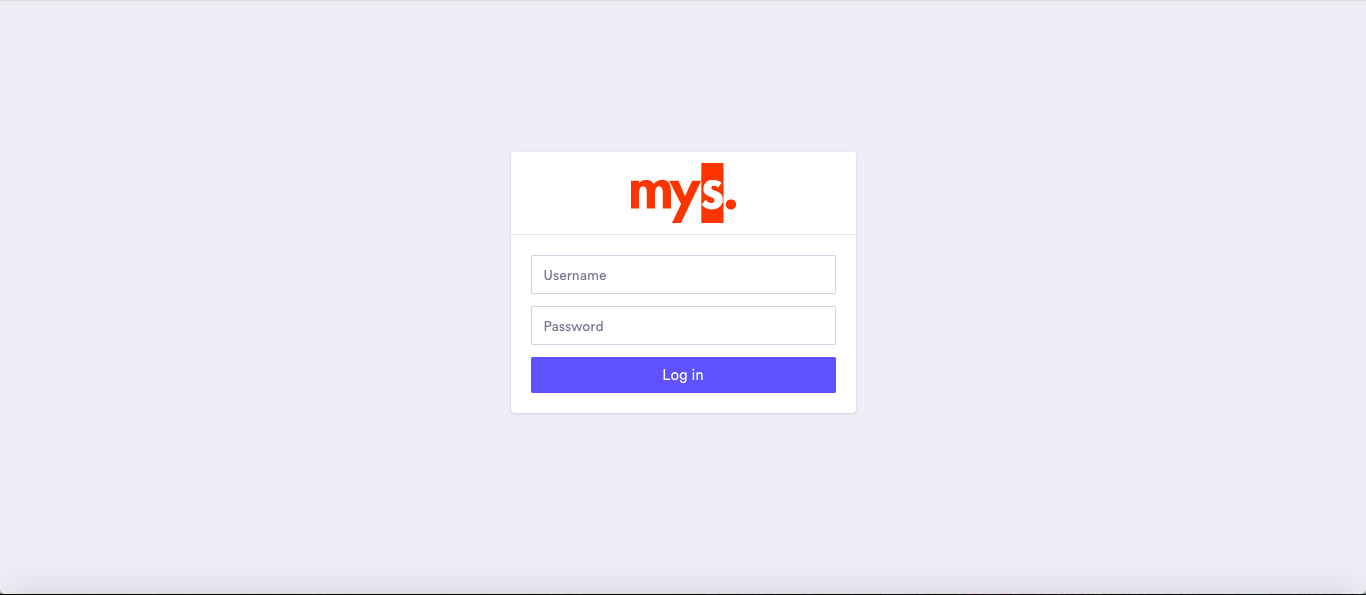
\includegraphics[scale = 0.3]{immagini/portale/login.png} 
	\caption {Portale Web, sezione di Login}
\end{figure}
\\Una volta effettuato il login, si viene reindirizzati al sito web, vero e proprio.\\
Da qui abbiamo principalmente 3 schermate principali:
\begin{itemize}
	\item Attrezzature;
	\item Calendario;
	\item Interventi.\\
\end{itemize}
La schermata Attrezzature mostra in forma tabellare, tutte le attrezzature e macchinari dell'azienda, con i vari dettagli.\\\\
La schermata Interventi mostra sempre in forma tabellare, i vari interventi richiesti su quale attrezzatura, e i dettagli dell'intervento.\\
E' presente un altra sezione, nella schermata Interventi, la sezione Interventi In Attesa, che mostra gli interventi che si stanno sincronizzando con il database SAP, che non sono ancora sincronizzati.
\newpage

\begin{figure}[!h] 
	\centering 
	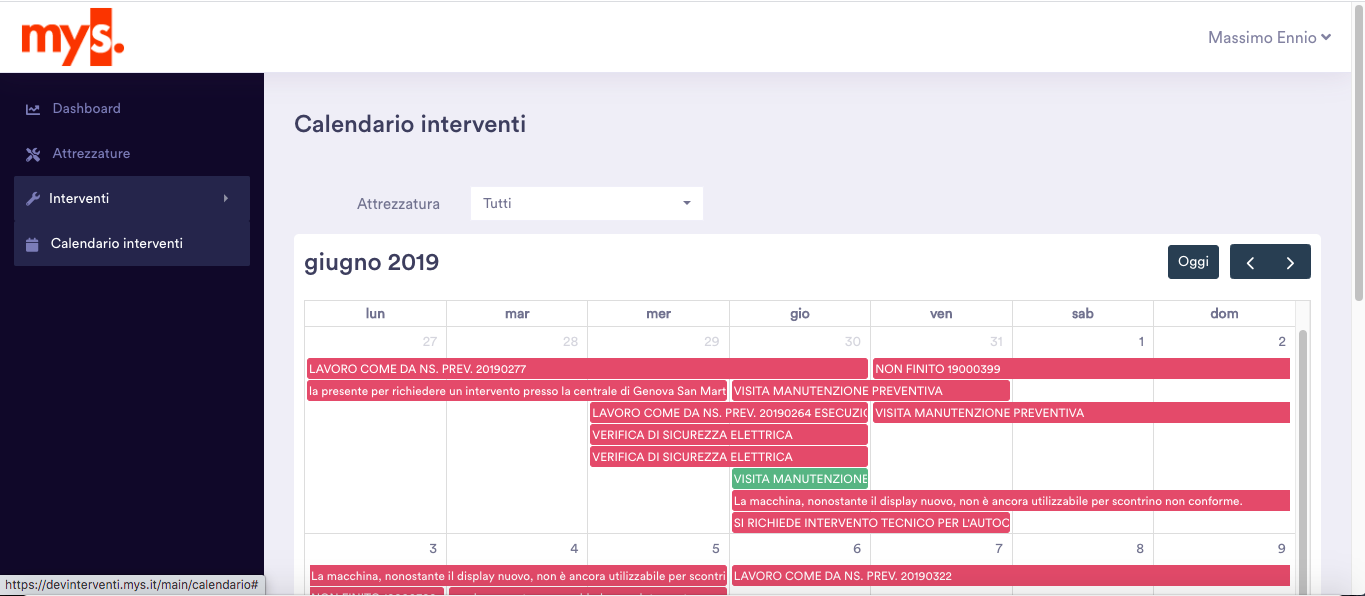
\includegraphics[scale = 0.3]{immagini/portale/calendario.png} 
	\caption {Portale Web, schermata Calendario}
	\label{fig:2-7}
\end{figure}
Cominciamo con la schermata Calendario, in figura \ref{fig:2-7}.\\
\\Evidenziate di rosso ci sono le chiamate di servizio, ad esempio manutenzioni, non completate, mentre evidenziate in verde quelle completate.\\\\
Ora continuiamo con la schermata Attrezzature.\\
\begin{figure}[!h] 
	\centering 
	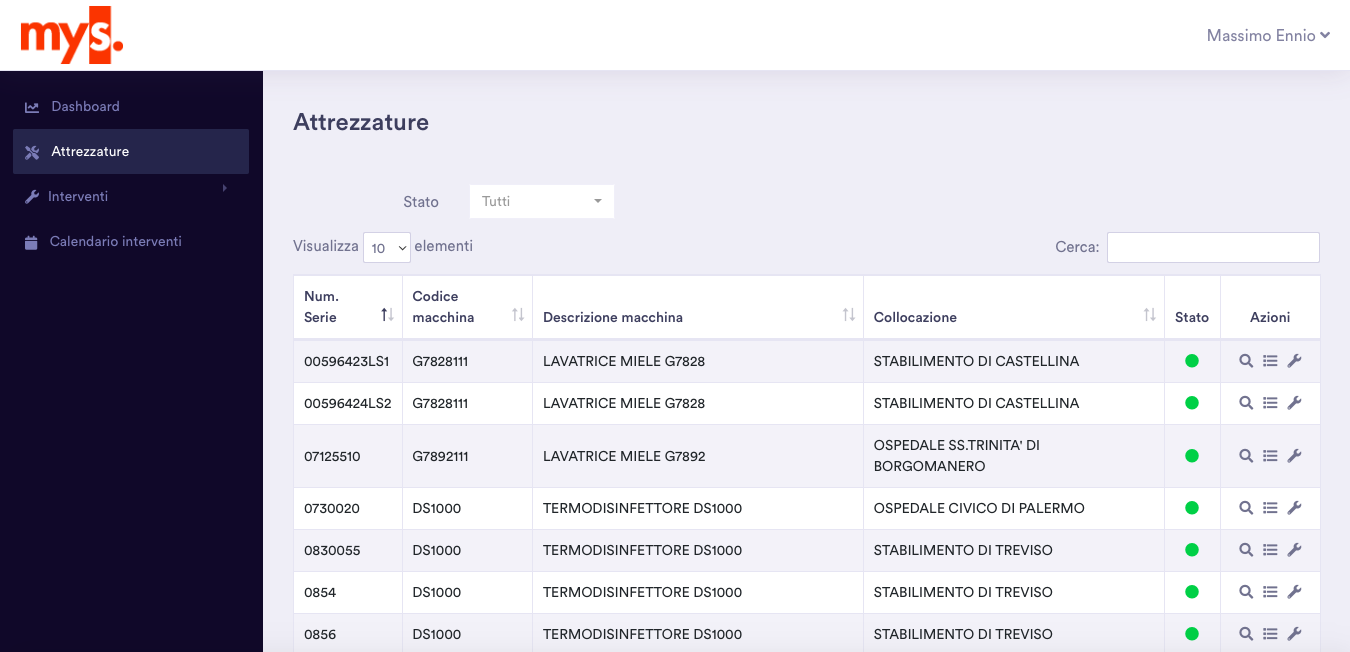
\includegraphics[scale = 0.25]{immagini/portale/attrezzature.png} 
	\caption {Portale Web, schermata Attrezzature}
	\label{fig:2-8}
\end{figure}
\\Nella figura \ref{fig:2-8} possiamo vedere tutte le attrezzature, relative all'azienda cliente collegata, e quindi alle credenziali.\\
Per ogni attrezzatura ci sono alcune azioni, tra cui ricerca ed elenco chiamate di servizio.\\Tra le varie azioni la più interessante è l'apertura di una nuova chiamata di servizio, ovvero richiedere un nuovo intervento, ad esempio una manutenzione o sostituzione di componenti.\\\\
Ora passiamo alla schermata degli interventi, di cui possiamo conoscerne tutte le caratteristiche principali, come numero e tipo di intervento, data inizio e fine.\\
E anche la causale e lo stato, per stato si intende se l'intervento è già stato effettuato.
\begin{figure}[!h] 
	\centering 
	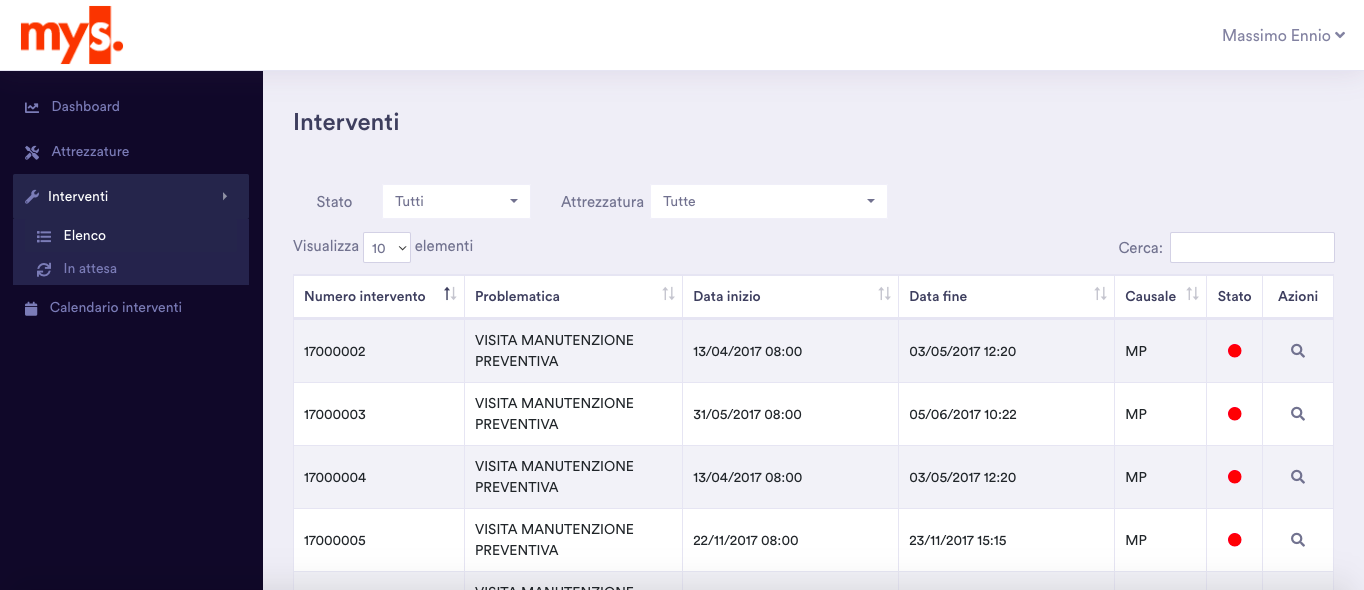
\includegraphics[scale = 0.25]{immagini/portale/interventi.png} 
	\caption {Portale Web, sezione di Login}
\end{figure}
\\\\Infine, all'interno della schermata degli interventi, abbiamo la sezione "In attesa", per gli interventi in attesa di sincronizzazione.\\
Questi sono gli interventi creati tramite questo portale web, che si stanno sincronizzando con il server SAP, lo stato verde indicano che si sono sincronizzati, quello rosso che non si sono ancora sincronizzati.
\begin{figure}[!h] 
	\centering 
	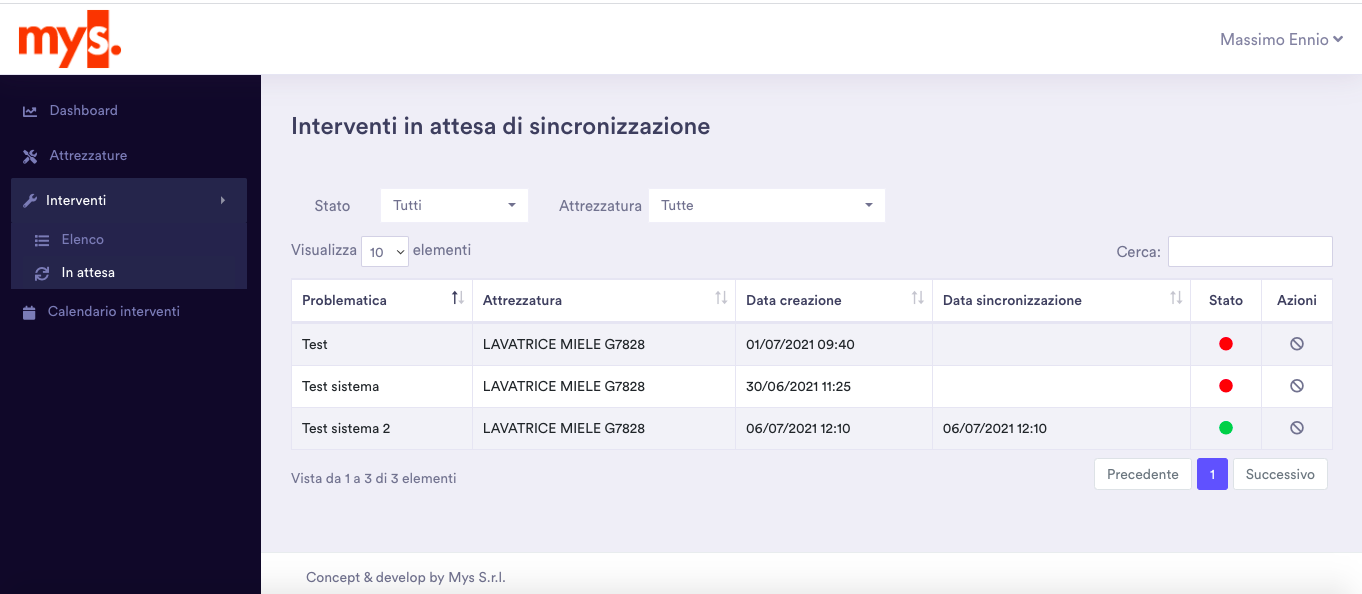
\includegraphics[scale = 0.25]{immagini/portale/interventi-in-attesa.png} 
	\caption {Portale Web, schermata Interventi, sezione In attesa}
\end{figure}
\pagebreak
\subsection{Webservices REST API}
\begin{flushleft}
	\item Recentemente, su SAP Business One è stato introdotto un service layer, composto da webservices REST API, che comunicano tramite protocollo ODATA (open data protocol).
	\item Questi webservices permettono di accedere direttamente agli oggetti SAP,\\senza passare per il client SAP.\\Gli oggetti SAP sono una struttura dati generata dalla logica del server SAP, \\che raggruppano e ordinano secondo certe logiche i dati presenti nel database.
	\\ Per poter ottenere questi dati bisogna fare una richiesta http al webserver, il quale invierà un file json con gli oggetti SAP richiesti.
	\\L'utilizzo più comune di questi webservices è un portale web che usi le informazioni prese tramite queste richieste HTTP. 
\end{flushleft}
\begin{figure}[!h] 
	\centering 
	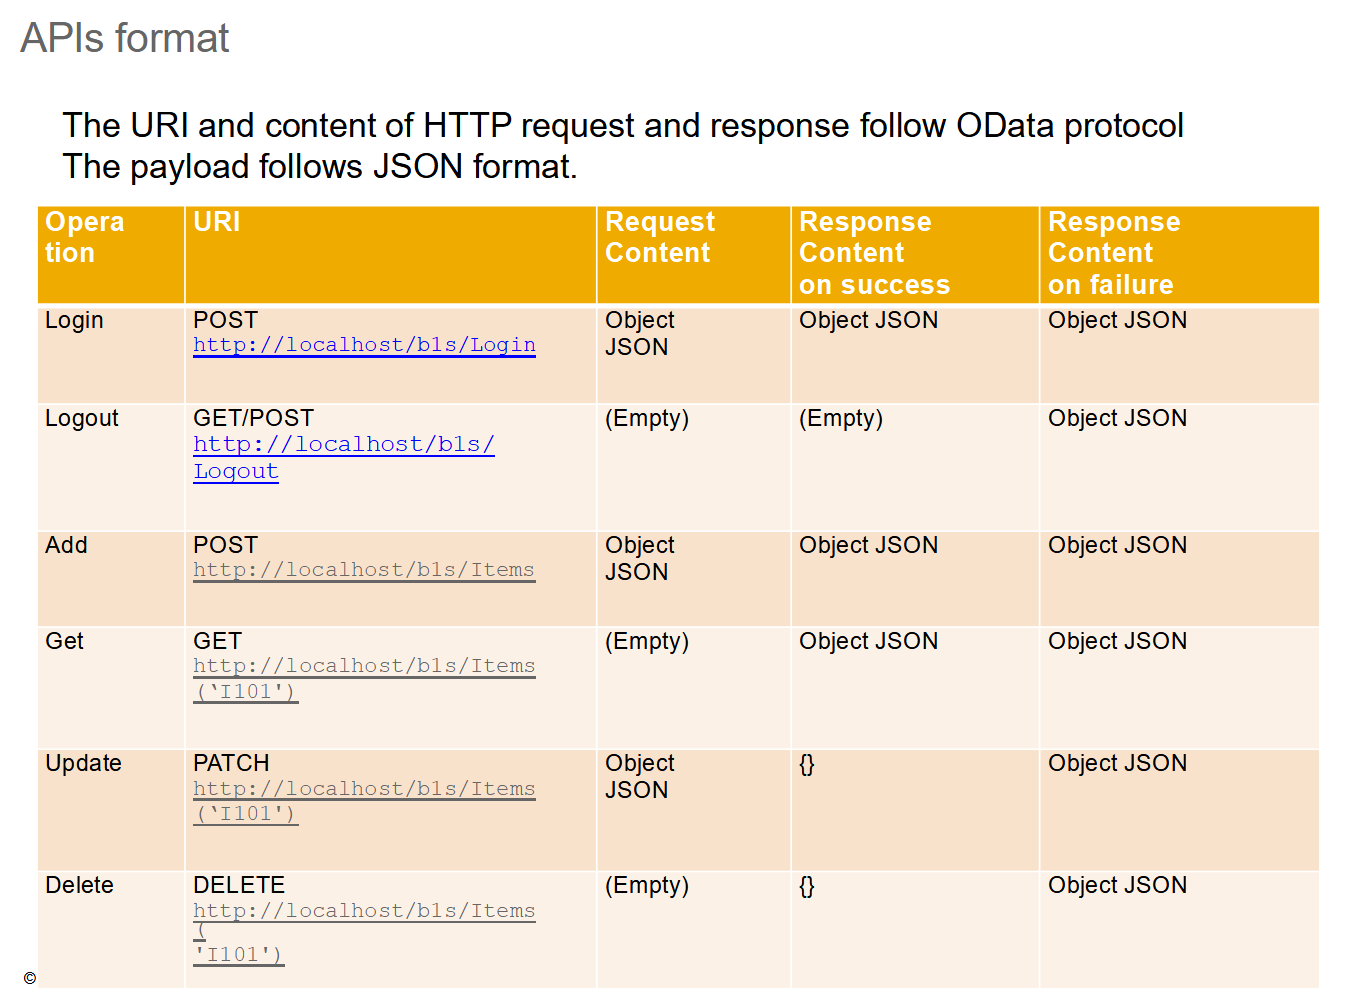
\includegraphics[scale = 0.37]{immagini/api_Format.png} 
	\caption {Formato delle richieste HTTP per il Service Layer SAP}
	\label{fig:2-11}
\end{figure}
\begin{flushleft}
	\item Come si può osservare in figura \ref{fig:2-11}, sono presenti le richieste HTTP principali per interagire con i webservices REST API del Service Layer di SAP.
	\item A seguito di una richiesta HTTP viene elaborata la richiesta.\\Viene restituito un oggetto JSON in caso di fallimento, comunicando l'errore causante il fallimento.\\In caso di successo viene restituito un oggetto JSON, ove necessario, oppure un messaggio vuote che rappresenta il successo dell'operazione.
\end{flushleft}
\section{Descrizione modulo MyService}
\begin{figure}[!h] 
	\centering 
	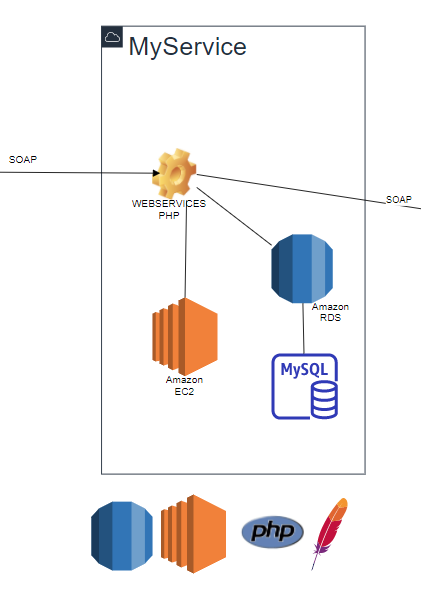
\includegraphics[scale = 1.1]{immagini/modulo-myservice.png} 
	\caption{Schema di rappresentazione modulo MyService dei servizi \gls{aws}}
	\label{fig:2-12}
\end{figure}
\newpage
\subsection{Servizi AWS}
In questo modulo abbiamo i webservices in PHP installati in un server \gls{aws}, accompagnato da un database MySQL.
\gls{aws} è un acronimo che sta per Amazon Web Services.
In particolare, dei servizi \gls{aws}, in questo modulo abbiamo:
\begin{itemize}
	\item Amazon \gls{ec2}, Amazon Elastic Compute Cloud, che consiste nel webserver, ovvero il server dove sono presenti i nostri webservices in php;
	\item Amazon \gls{rds}, Amazon Relational Database Service, che si occupa della gestione del database MySQL;
	\item Amazon \gls{s3}, Amazon Simple Storage Service, che nello schema non è presente, ma si occupa della gestione di allegati e file troppo pesanti nel database per essere gestiti da Amazon \gls{rds}.
\end{itemize}
Ora rivolgiamo la nostra attenzione ai webservices PHP, che mettono in relazione questo webserver e il database con il modulo SAP e il modulo MySapp, delle applicazioni mobile, attraverso il protocollo \gls{soap}.
\subsection{Webservices PHP}
Come possiamo vedere dalle figure \ref{fig:2-11} e \ref{2-1}, il client SAP comunica con questi webservices PHP, attraverso un add-on che utilizza il protocollo \gls{soap}.\\
Per programmare questi webservices sono state utilizzate le tecnologie Apache e PHP.\\ 
Il protocollo \gls{soap}, ovvero Simple Object Access Protocol, è un protocollo per lo scambio di messaggi tra componenti software.\\\\
I webservices php comunicano anche con le applicazioni mobile, per Android e iOS, sempre tramite protocollo \gls{soap}.\\
Vi sono moltissime funzioni in PHP che corrispondono a molte funzioni \gls{soap} nei webservices, il cui compito principale è mettere in relazione le app mobile o il SAP, con il database contenuto in questo modulo.\\
L'obiettivo principale è gestire le chiamate di servizio, ovvero richieste di intervento, ai tecnici del SAP.\\
Elenchiamo alcune delle funzioni più comuni:
\begin{itemize}
	\item Visione di tutti i dettagli di una chiamata di servizio;
	\item Visione di tutte le chiamate di servizio di un tecnico;
	\item Rimozione di una chiamata di servizio;
	\item Modifica di una chiamata di servizio;
	\item Aggiunta di una chiamata di servizio;
	\item Invio mail a cliente, una volta concluso una chiamata di servizio;
	\item Login di un tecnico;
	\item Logout di un tecnico.
\end{itemize}
\newpage
\section{Descrizione modulo MySapp}
\begin{figure}[!h] 
	\centering 
	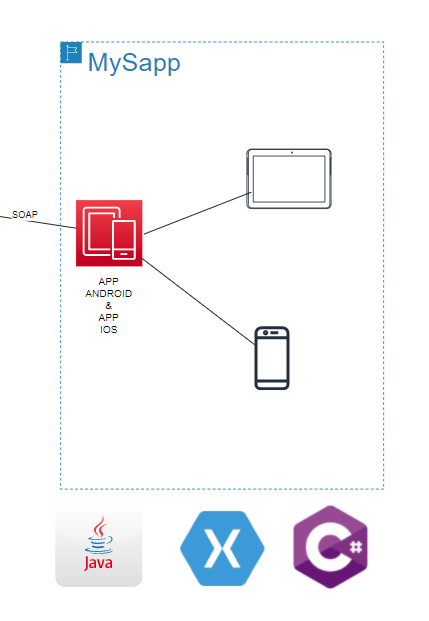
\includegraphics[scale = 1.1]{immagini/modulo-mysapp.png} 
	\caption{Schema di rappresentazione modulo MySapp delle applicazioni mobili}
\end{figure}
\newpage
\subsection{Applicazioni mobile}
Il modulo MyService si collega con questo modulo MySapp, attraverso il protocollo \gls{soap} utilizzando i webservices PHP del modulo MyService.\\
Sono state sviluppate due applicazioni per i clienti che risolvono le chiamate di servizio on-site, ovvero di persona.\\
In queste applicazioni, il tecnico esegue il login, con le sue credenziali e successivamente può gestire le chiamate di servizio a egli assegnate.\\
Ora vediamo velocemente com'è stato impostato il layout delle due applicazioni.
\subsubsection{Applicazione iOS}
Per lo sviluppo dell'applicazione iOS è stato utilizzando C\# e Xamarin.\\\\
Cominciamo con la schermata di login.\\
\begin{figure}[!h] 
	\centering 
	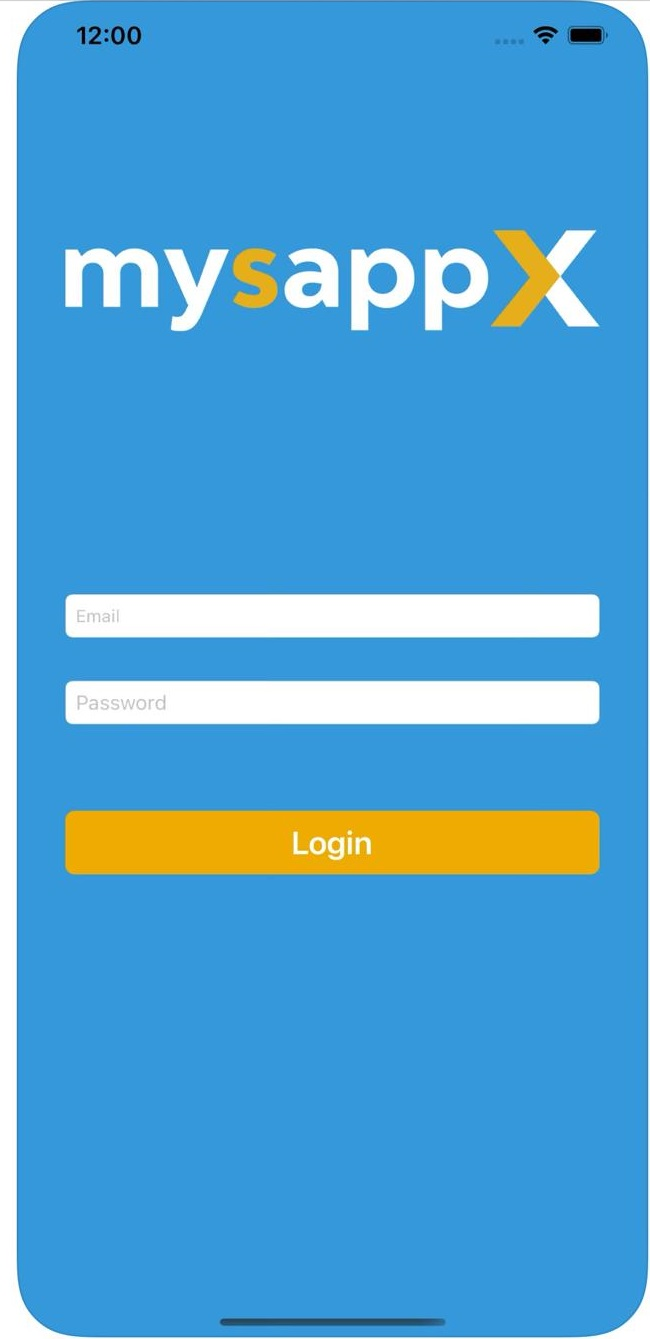
\includegraphics[scale = 0.2]{immagini/app iOS/login-iOS.jpeg} 
	\caption {App iOS, schermata di Login}
	\label{fig:2-14}
\end{figure}
\\In figura \ref{fig:2-14} il tecnico dovrà inserire le proprie credenziali e accederà alla gestione delle chiamate di servizio a lui assegnate.
\newpage
\begin{flushleft}
	Continuiamo con la schermata Principale dell'app.
	\\In questa schermata si possono vedere le chiamate di servizio assegnate a questo tecnico ancora da eseguire.
\end{flushleft}
\begin{figure}[!h] 
	\centering 
	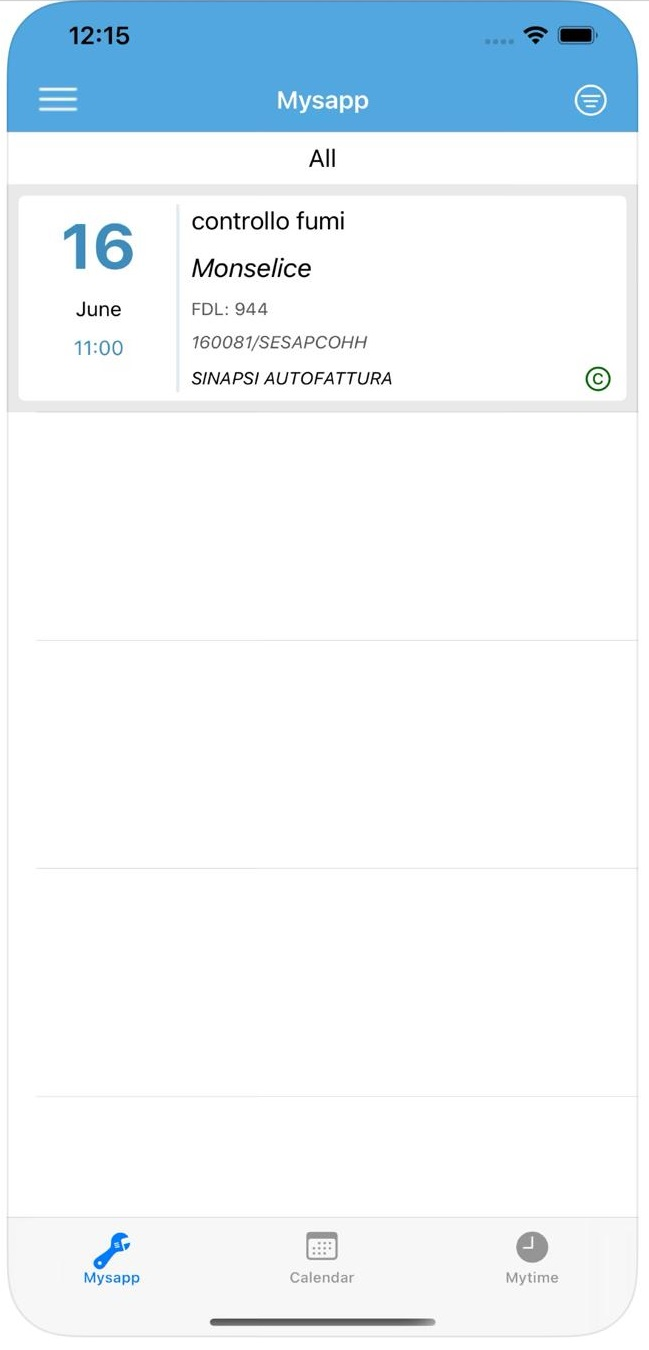
\includegraphics[scale = 0.13]{immagini/app iOS/elenco-interventi-iOS.jpeg} 
	\caption {App iOS, schermata Principale}
	\label{fig:2-15}
\end{figure}
In figura \ref{fig:2-15} possiamo vedere il calendario e la posizione della o delle chiamate di servizio da eseguire.\\
\begin{figure}[!h] 
	\centering 
	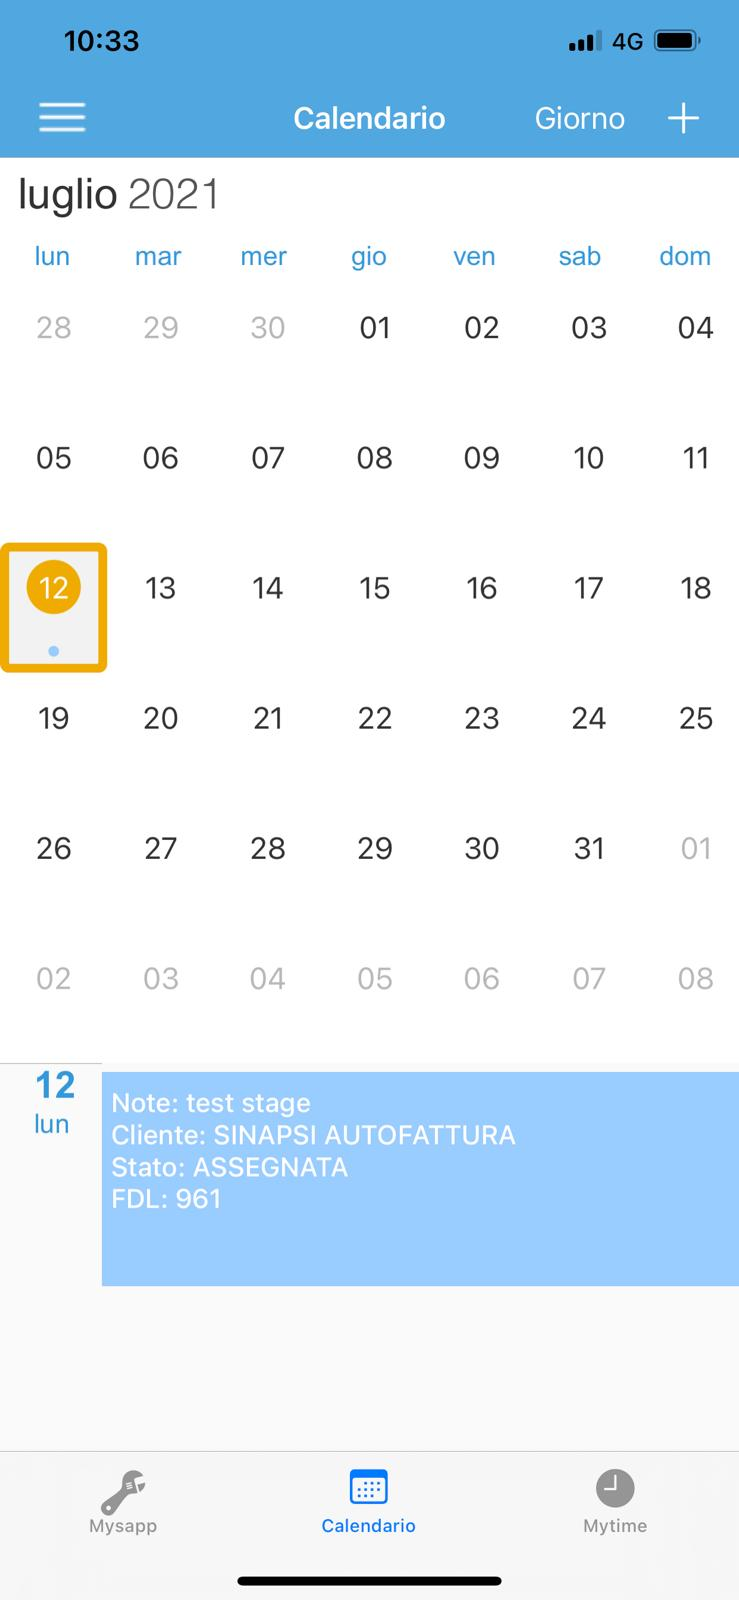
\includegraphics[scale = 0.13]{immagini/app iOS/calendario-iOS.jpeg} 
	\caption {App iOS, schermata Calendario}
\end{figure}
\newpage

\begin{figure}[!h] 
	\centering 
	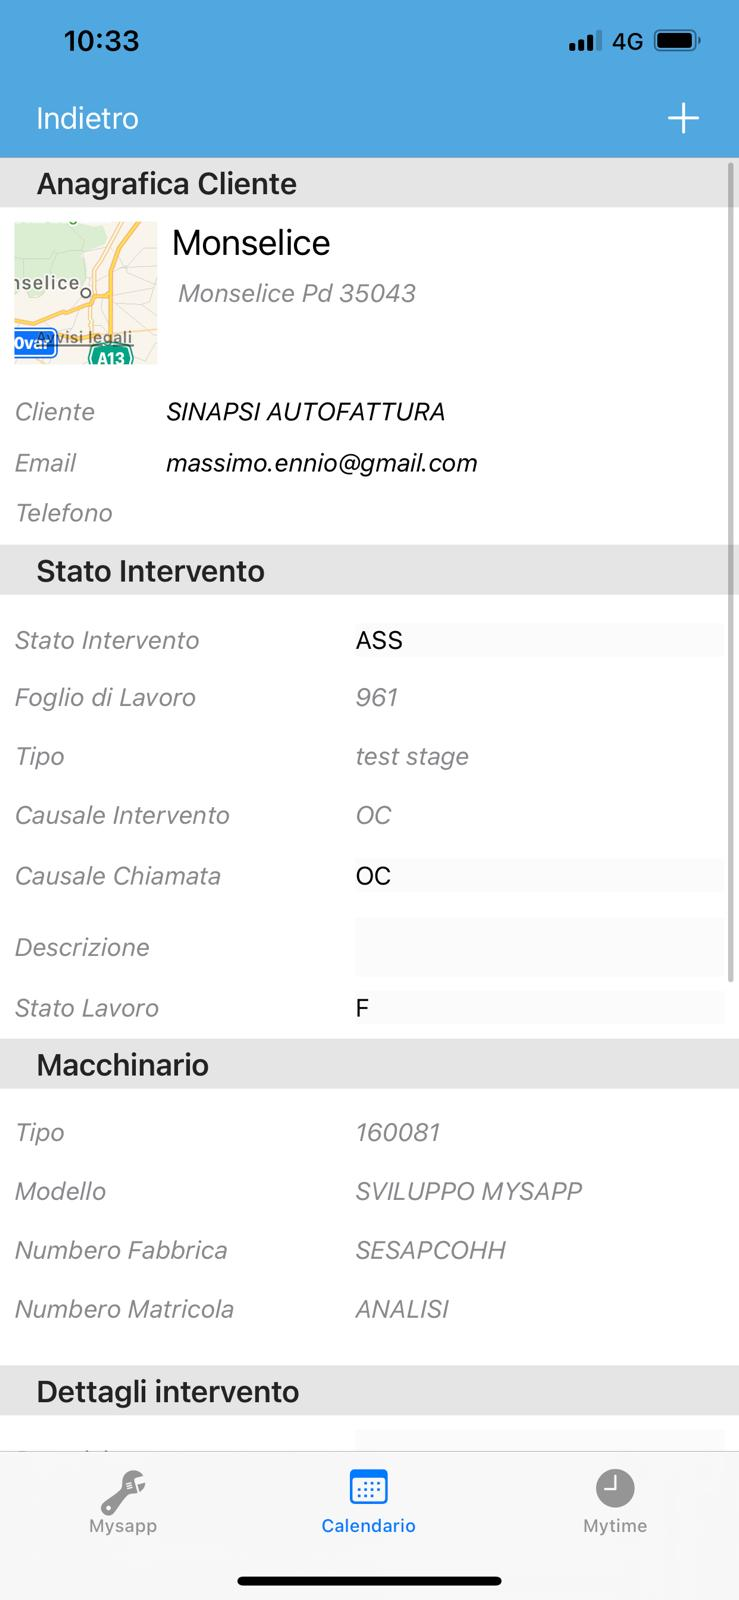
\includegraphics[scale = 0.2]{immagini/app iOS/intervento-iOS.jpeg} 
	\caption {App iOS, schermata Intervento}
	\label{fig:2-17}
\end{figure}
Infine, in figura \ref{fig:2-17} abbiamo i dettagli della chiamata di servizio selezionata, dove possiamo vedere i vari dettagli della chiamata di servizio, ad esempio:
\begin{itemize}
	\item posizione del cliente;
	\item stato dell'intervento;
	\item attrezzatura che necessita dell'intervento;
	\item e altri dettagli meno importanti.
\end{itemize}
\newpage
\subsubsection{Applicazione Android}
Per lo sviluppo dell'applicazione Android è stato utilizzato Java e Kotlin.\\\\
Cominciamo a esplorare l'applicazione dalla schermata di login.\\
\begin{figure}[!h] 
	\centering 
	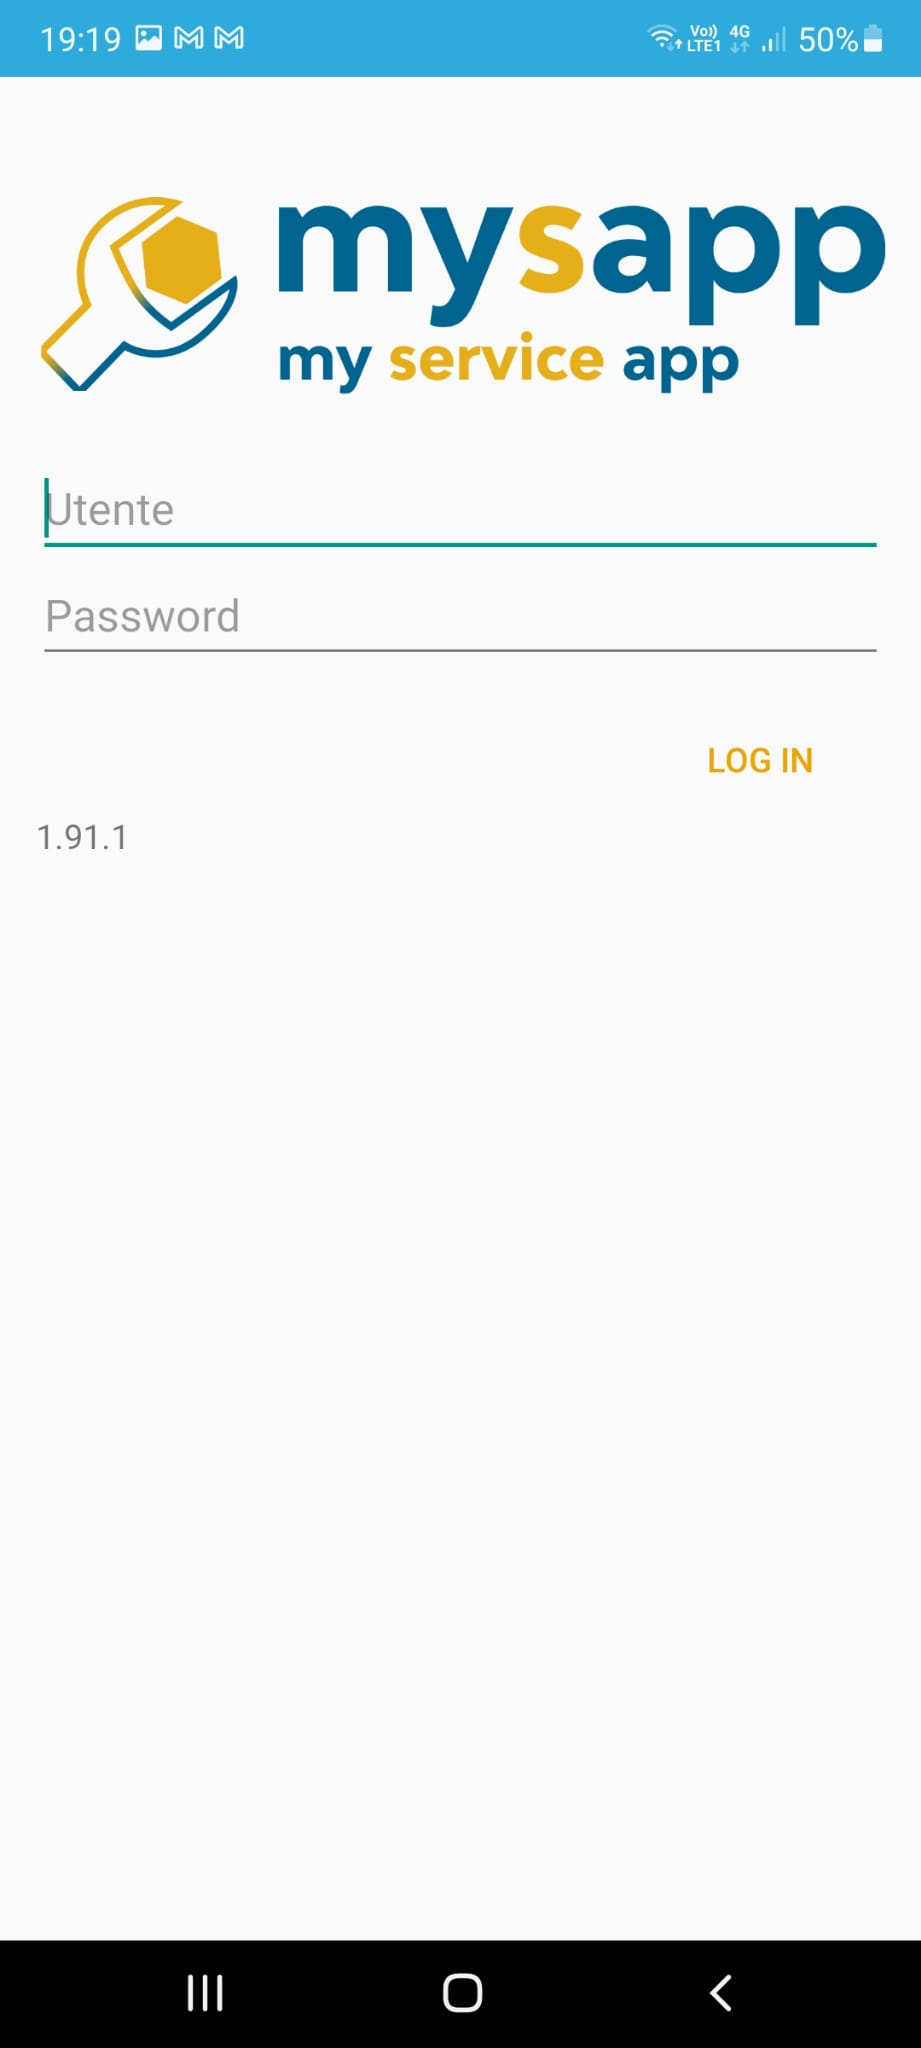
\includegraphics[scale = 0.2]{immagini/app Android/login-android.jpeg} 
	\caption {App Android, schermata di Login}
	\label{fig:2-18}
\end{figure}
In figura \ref{fig:2-18} il tecnico dovrà inserire le proprie credenziali.\\
\newpage
\begin{figure}[!h] 
	\centering 
	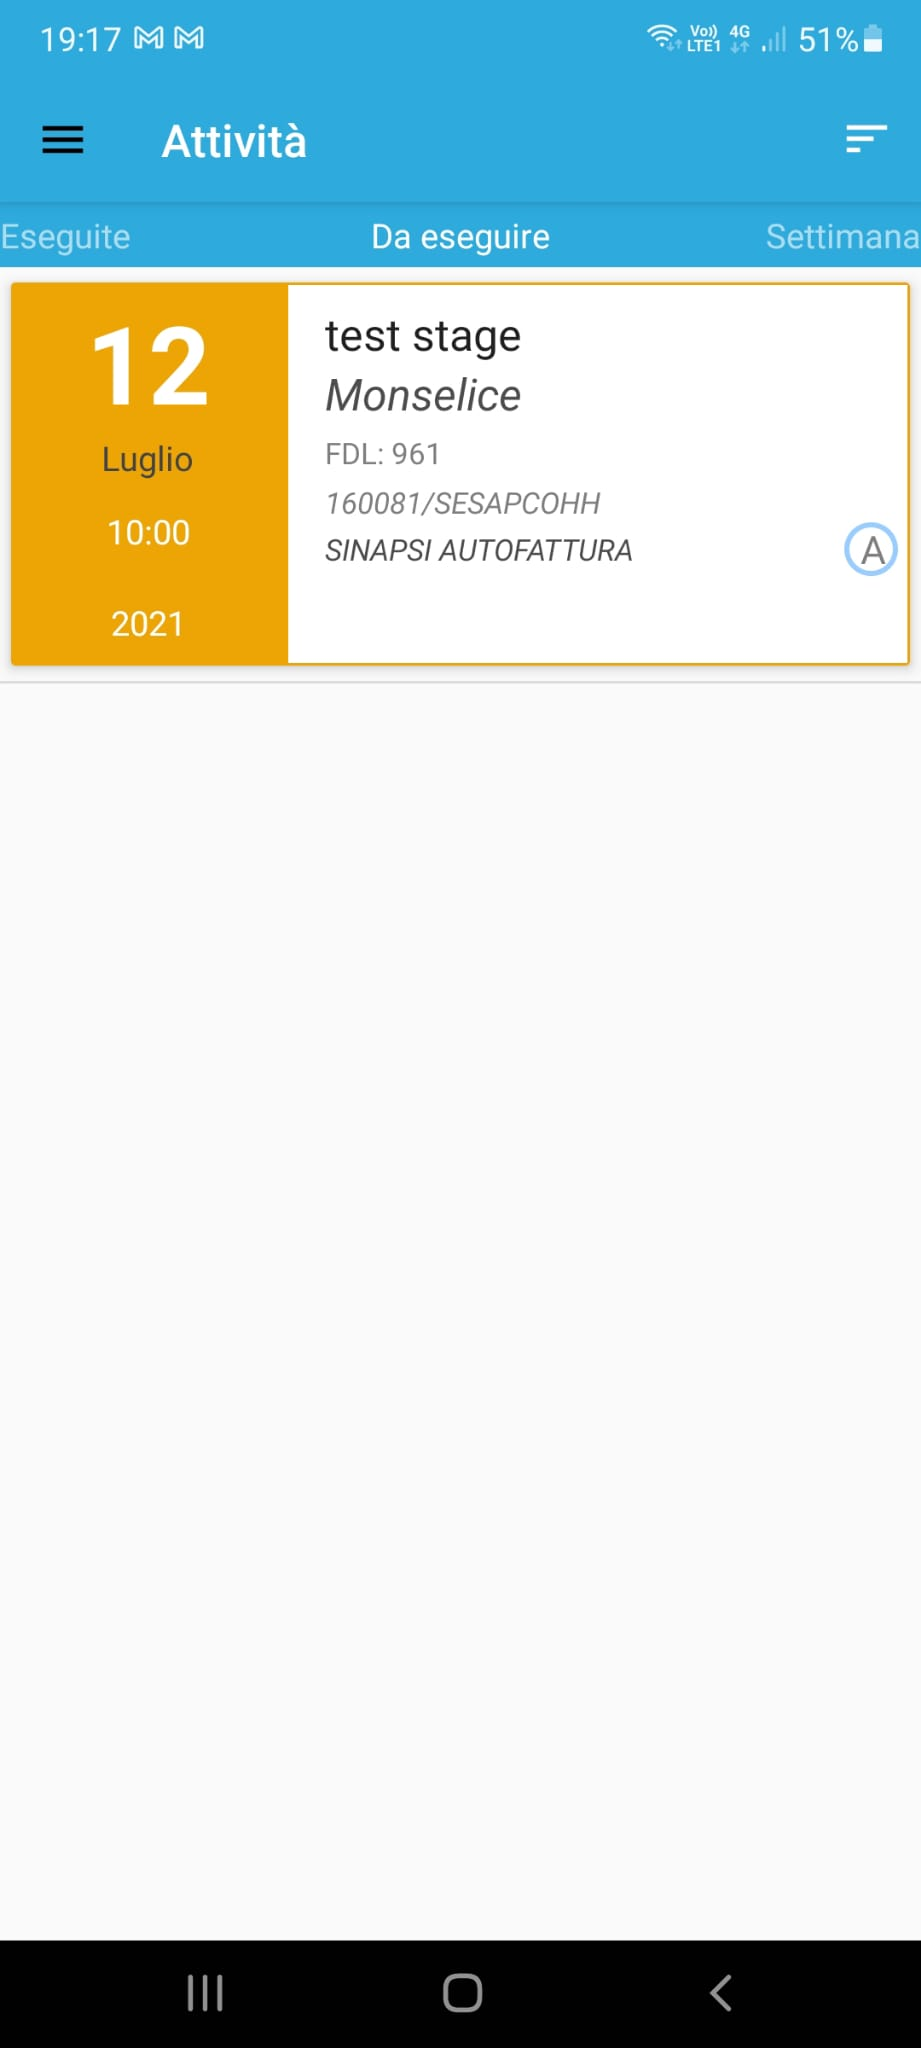
\includegraphics[scale = 0.11]{immagini/app Android/elenco-interventi-android.jpeg} 
	\caption {App Android, schermata Principale}
	\label{fig:2-19}
\end{figure}
In figura \ref{fig:2-19} possiamo vedere la schermata Principale dell'app, dove si possono vedere le chiamate assegnate al tecnico che ha eseguito l'accesso nell'applicazione.
\begin{figure}[!h] 
	\centering 
	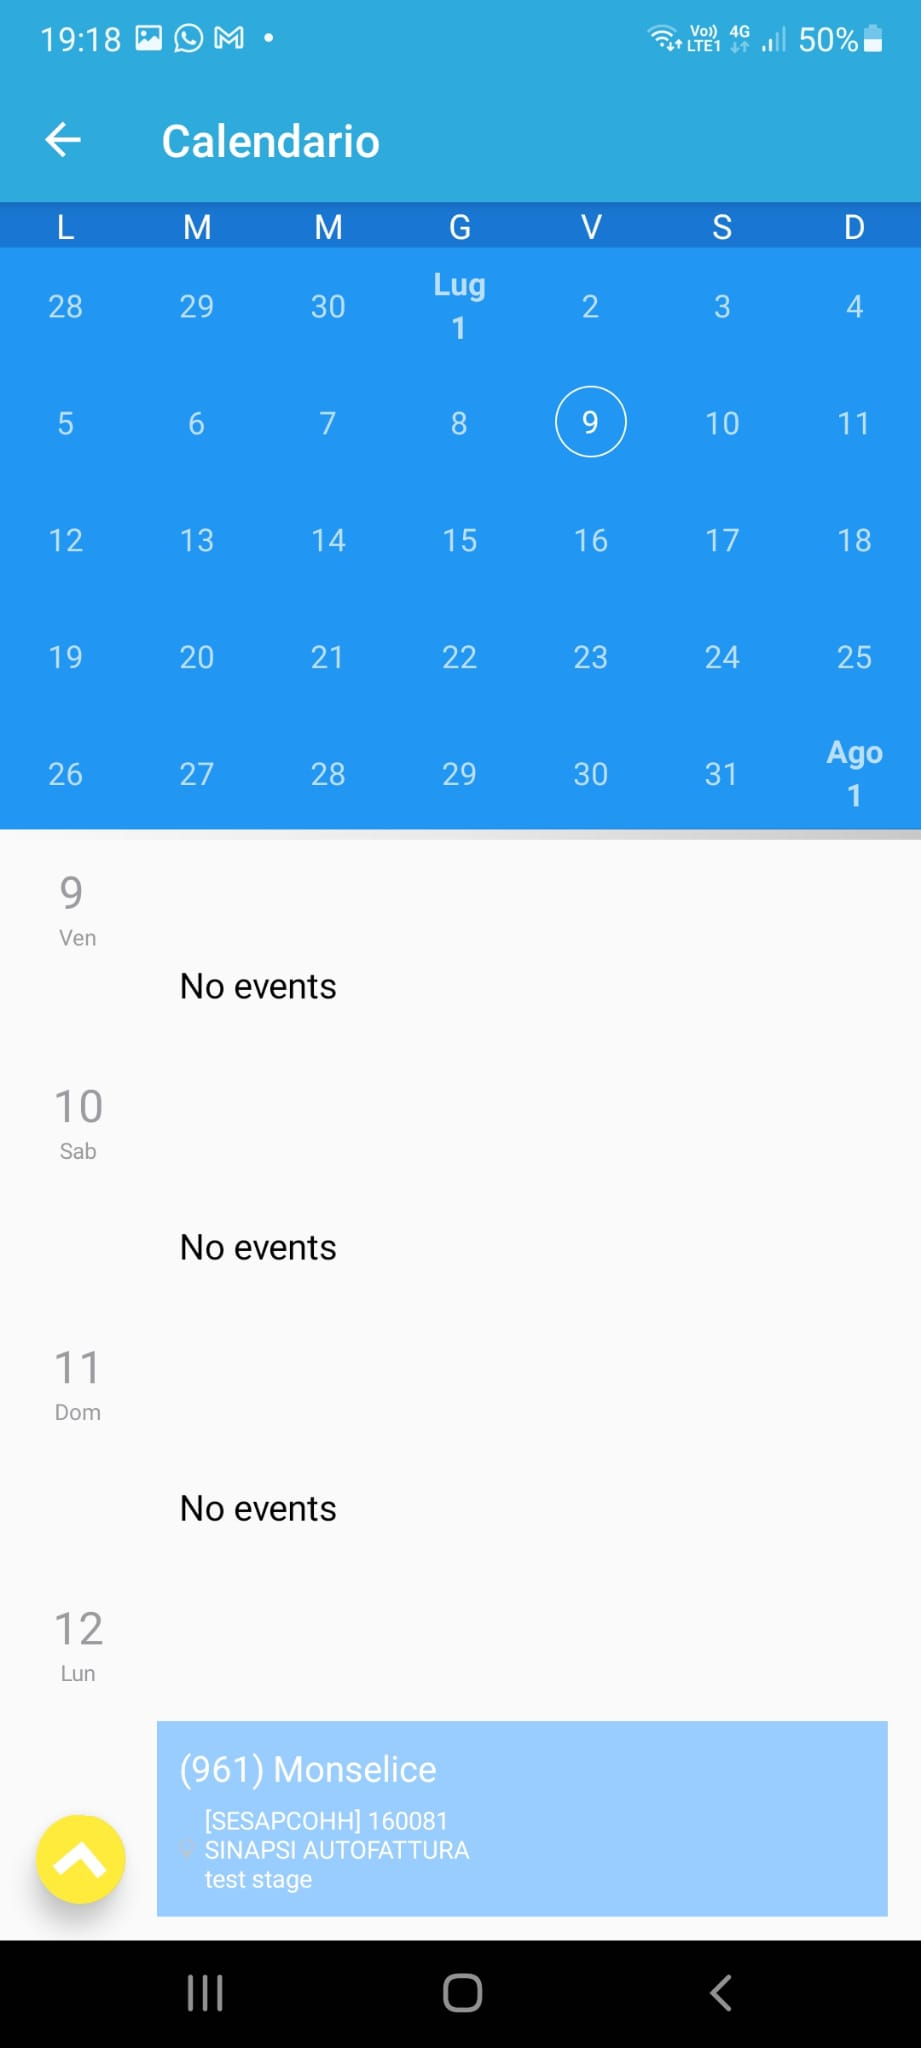
\includegraphics[scale = 0.11]{immagini/app Android/calendario-android.jpeg}
	\caption {App Android, schermata Calendario}
	\label{fig:2-20}
\end{figure}
In figura \ref{fig:2-20} possiamo vedere la schermata calendario dell'app.\\
\newpage
Infine, abbiamo i dettagli della chiamata di servizio selezionata.\\
\begin{figure}[!h] 
	\centering 
	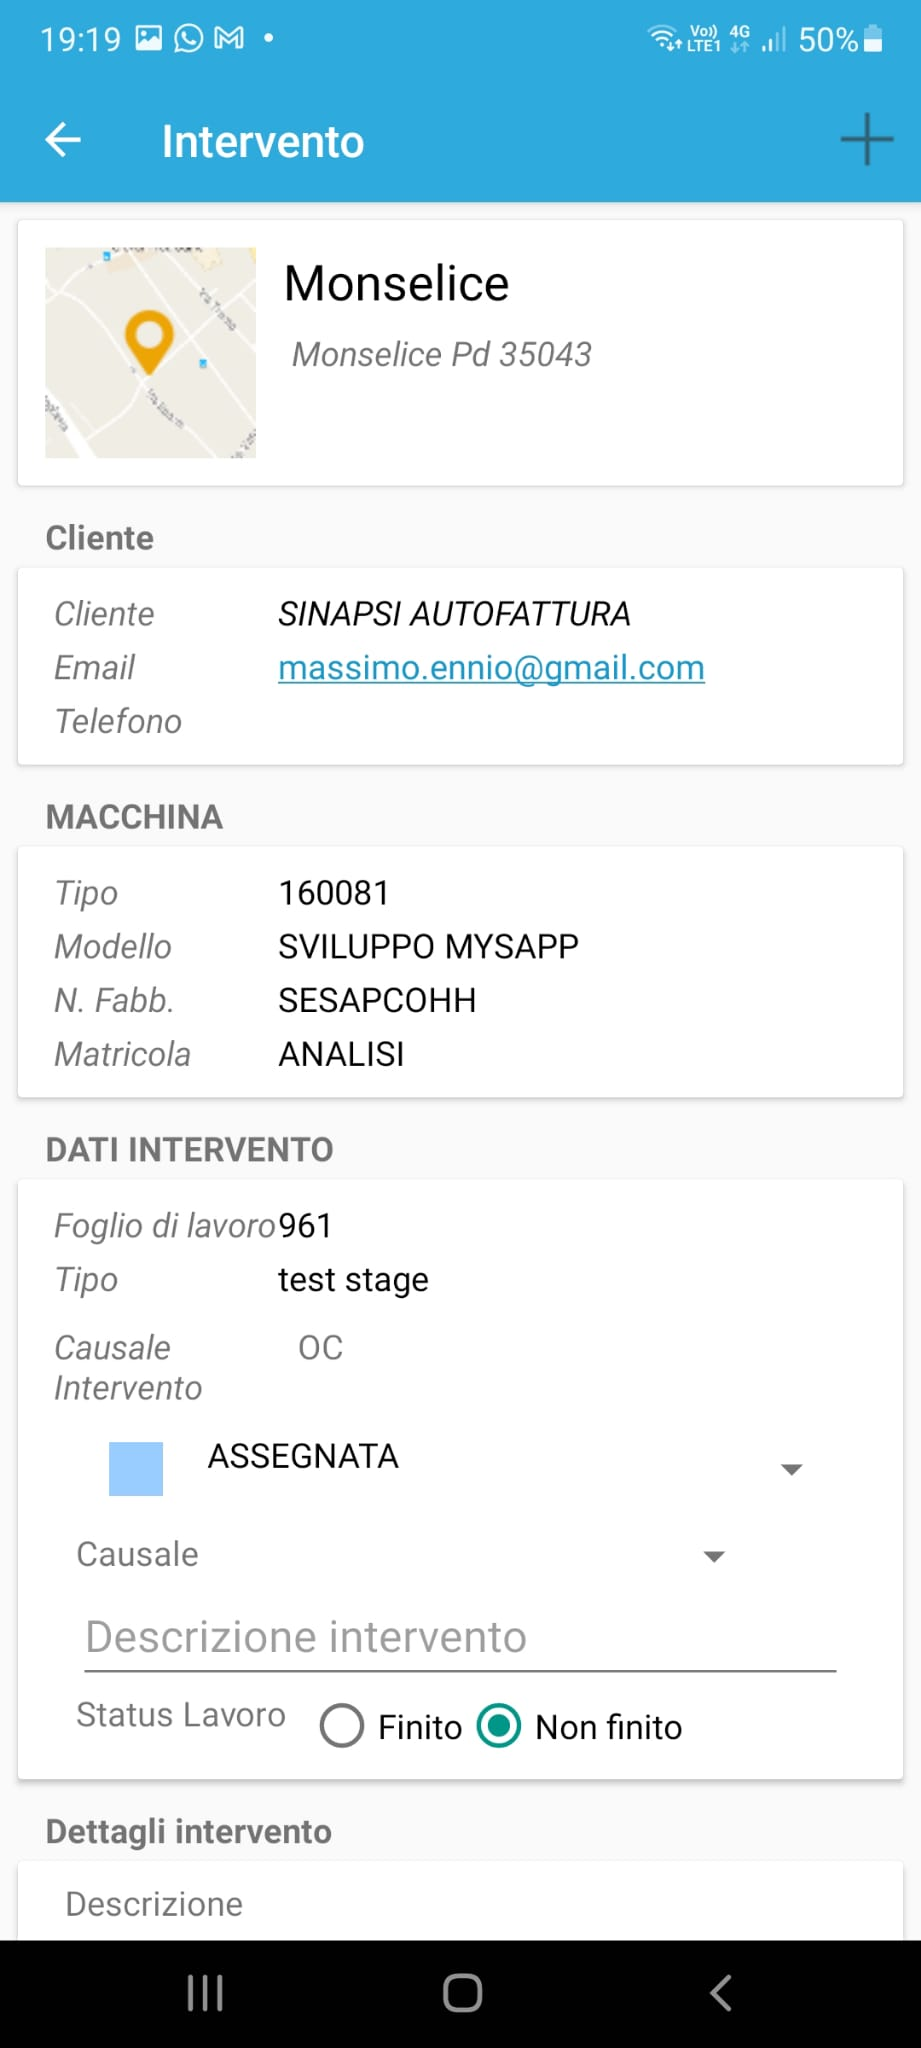
\includegraphics[scale = 0.2]{immagini/app Android/intervento-android.jpeg} 
	\caption {App Android, schermata Intervento}
	\label{fig:2-21}
\end{figure}
\\In figura \ref{fig:2-21} possiamo vedere i vari dettagli della chiamata di servizio, ad esempio:
\begin{itemize}
	\item posizione del cliente;
	\item attrezzatura che necessita dell'intervento;
	\item dati e dettagli dell'intervento.
\end{itemize}
\newpage
\section{Tecnologie coinvolte}
In questa sezione approfondiremo le tecnologie coinvolte durante lo stage:
\begin{itemize}
    \item {\textbf{PHP:}} Insieme ad Apache viene utilizzato per sviluppare applicazioni web lato server.
	
	In questo caso, viene utilizzato dall'azienda per lo sviluppo e gestione dei webservice sui server \gls{aws}.
	\item {\textbf{VB.NET:}} Linguaggio di programmazione per programmare gli add-ons, su Visual Studio, utilizzando le librerie \gls{sapb1}.
	\item {\textbf{C\#:}} Linguaggio di programmazione alternativo per programmare gli add-ons.
	
	Sempre su Visual Studio, utilizzando le librerie fornite dalla \gls{sapb1} SDK.
    \item {\textbf{SoapUI:}} Applicazione utilizzata per testare ed interagire con i webservices PHP, con protocollo \gls{soap}.
	
	E' possibile inserire una chiamata e l'applicazione ritorna una risposta dopo aver interagito con i webservice.
    \item {\textbf{HeidiSQL:}} Strumento di gestione di databases, quali MySQL, MariaDB, InnoDB.
	
	In questo caso utilizzato per il database MySQL del server \gls{aws}, per controllare che le operazioni di webservices modifichino o meno il database.
    \item {\textbf{MIcrosoft Visual Studio:}} Strumento di sviluppo software, \gls{ide}, utilizzato per programmare codice di vario tipo, da applicazione desktop ad app mobile, e raramente utilizzato per applicazioni web.
	
	In questo caso necessario per programmare gli add-ons, poichè le librerie necessarie sono predisposte per Visual Studio.
	\item {\textbf{Microsoft SQL Server Management Studio (SSMS):}} Applicazione utilizzata per gestire i database, viene utilizzata particolarmente per i server SQL Server.
	
	Nel nostro caso l'applicazione viene utilizzata per accedere direttamente ai database del server SAP.
	\item {\textbf{Remote Desktop:}} Applicazione preinstallata su Windows per accedere ad altri computer nella stessa rete locale.
	
	Viene utilizzata per accedere ai server SAP, presenti nella rete locale aziendale.
	\item {\textbf{Domino Lotus Notes:}} Applicazione utilizzata principalmente per la mail aziendale.
	
	Contiene però altre funzionalità quali un calendario aziendale e un server condiviso (domino) aziendale, che comprende database di fatture e password per accedere a diversi software aziendali o di clienti dell'azienda.
    \item {\textbf{Postman:}} Applicazione utilizzata per gestire e testare le API.
    
    Nel caso dell'azienda è stata utilizzata principalmente per controllare il corretto funzionamento e testare nuovi tipi di richieste sui webservices REST API di \gls{sapb1}.
\end{itemize} 
